\appendix
\chapter{Class diagram} \label{appendix-class}
\begin{figure}[h]
	\begin{center}
		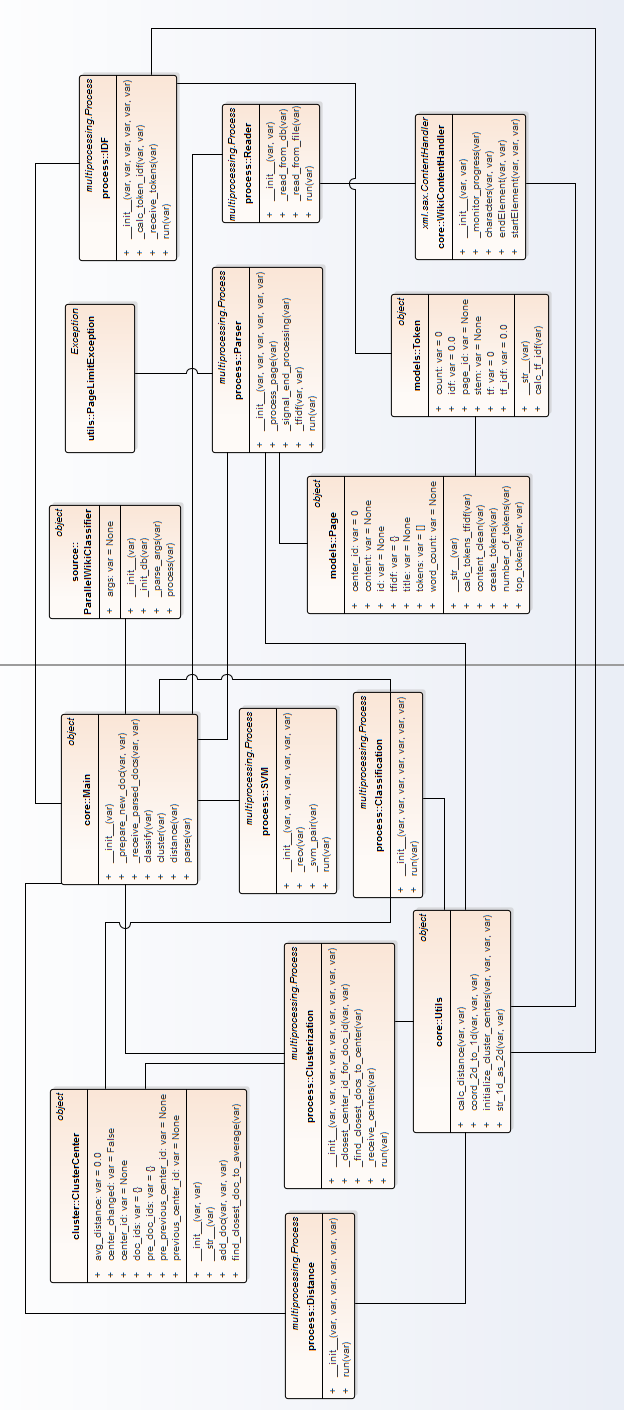
\includegraphics[width=0.72\linewidth]{images/diagrams/class3svm-h.png}
		\label{appendix-class-diagram}
	\end{center}
\end{figure}

\chapter{Sequence diagram} \label{appendix-sequence}
\begin{figure}[h]
	\begin{center}
		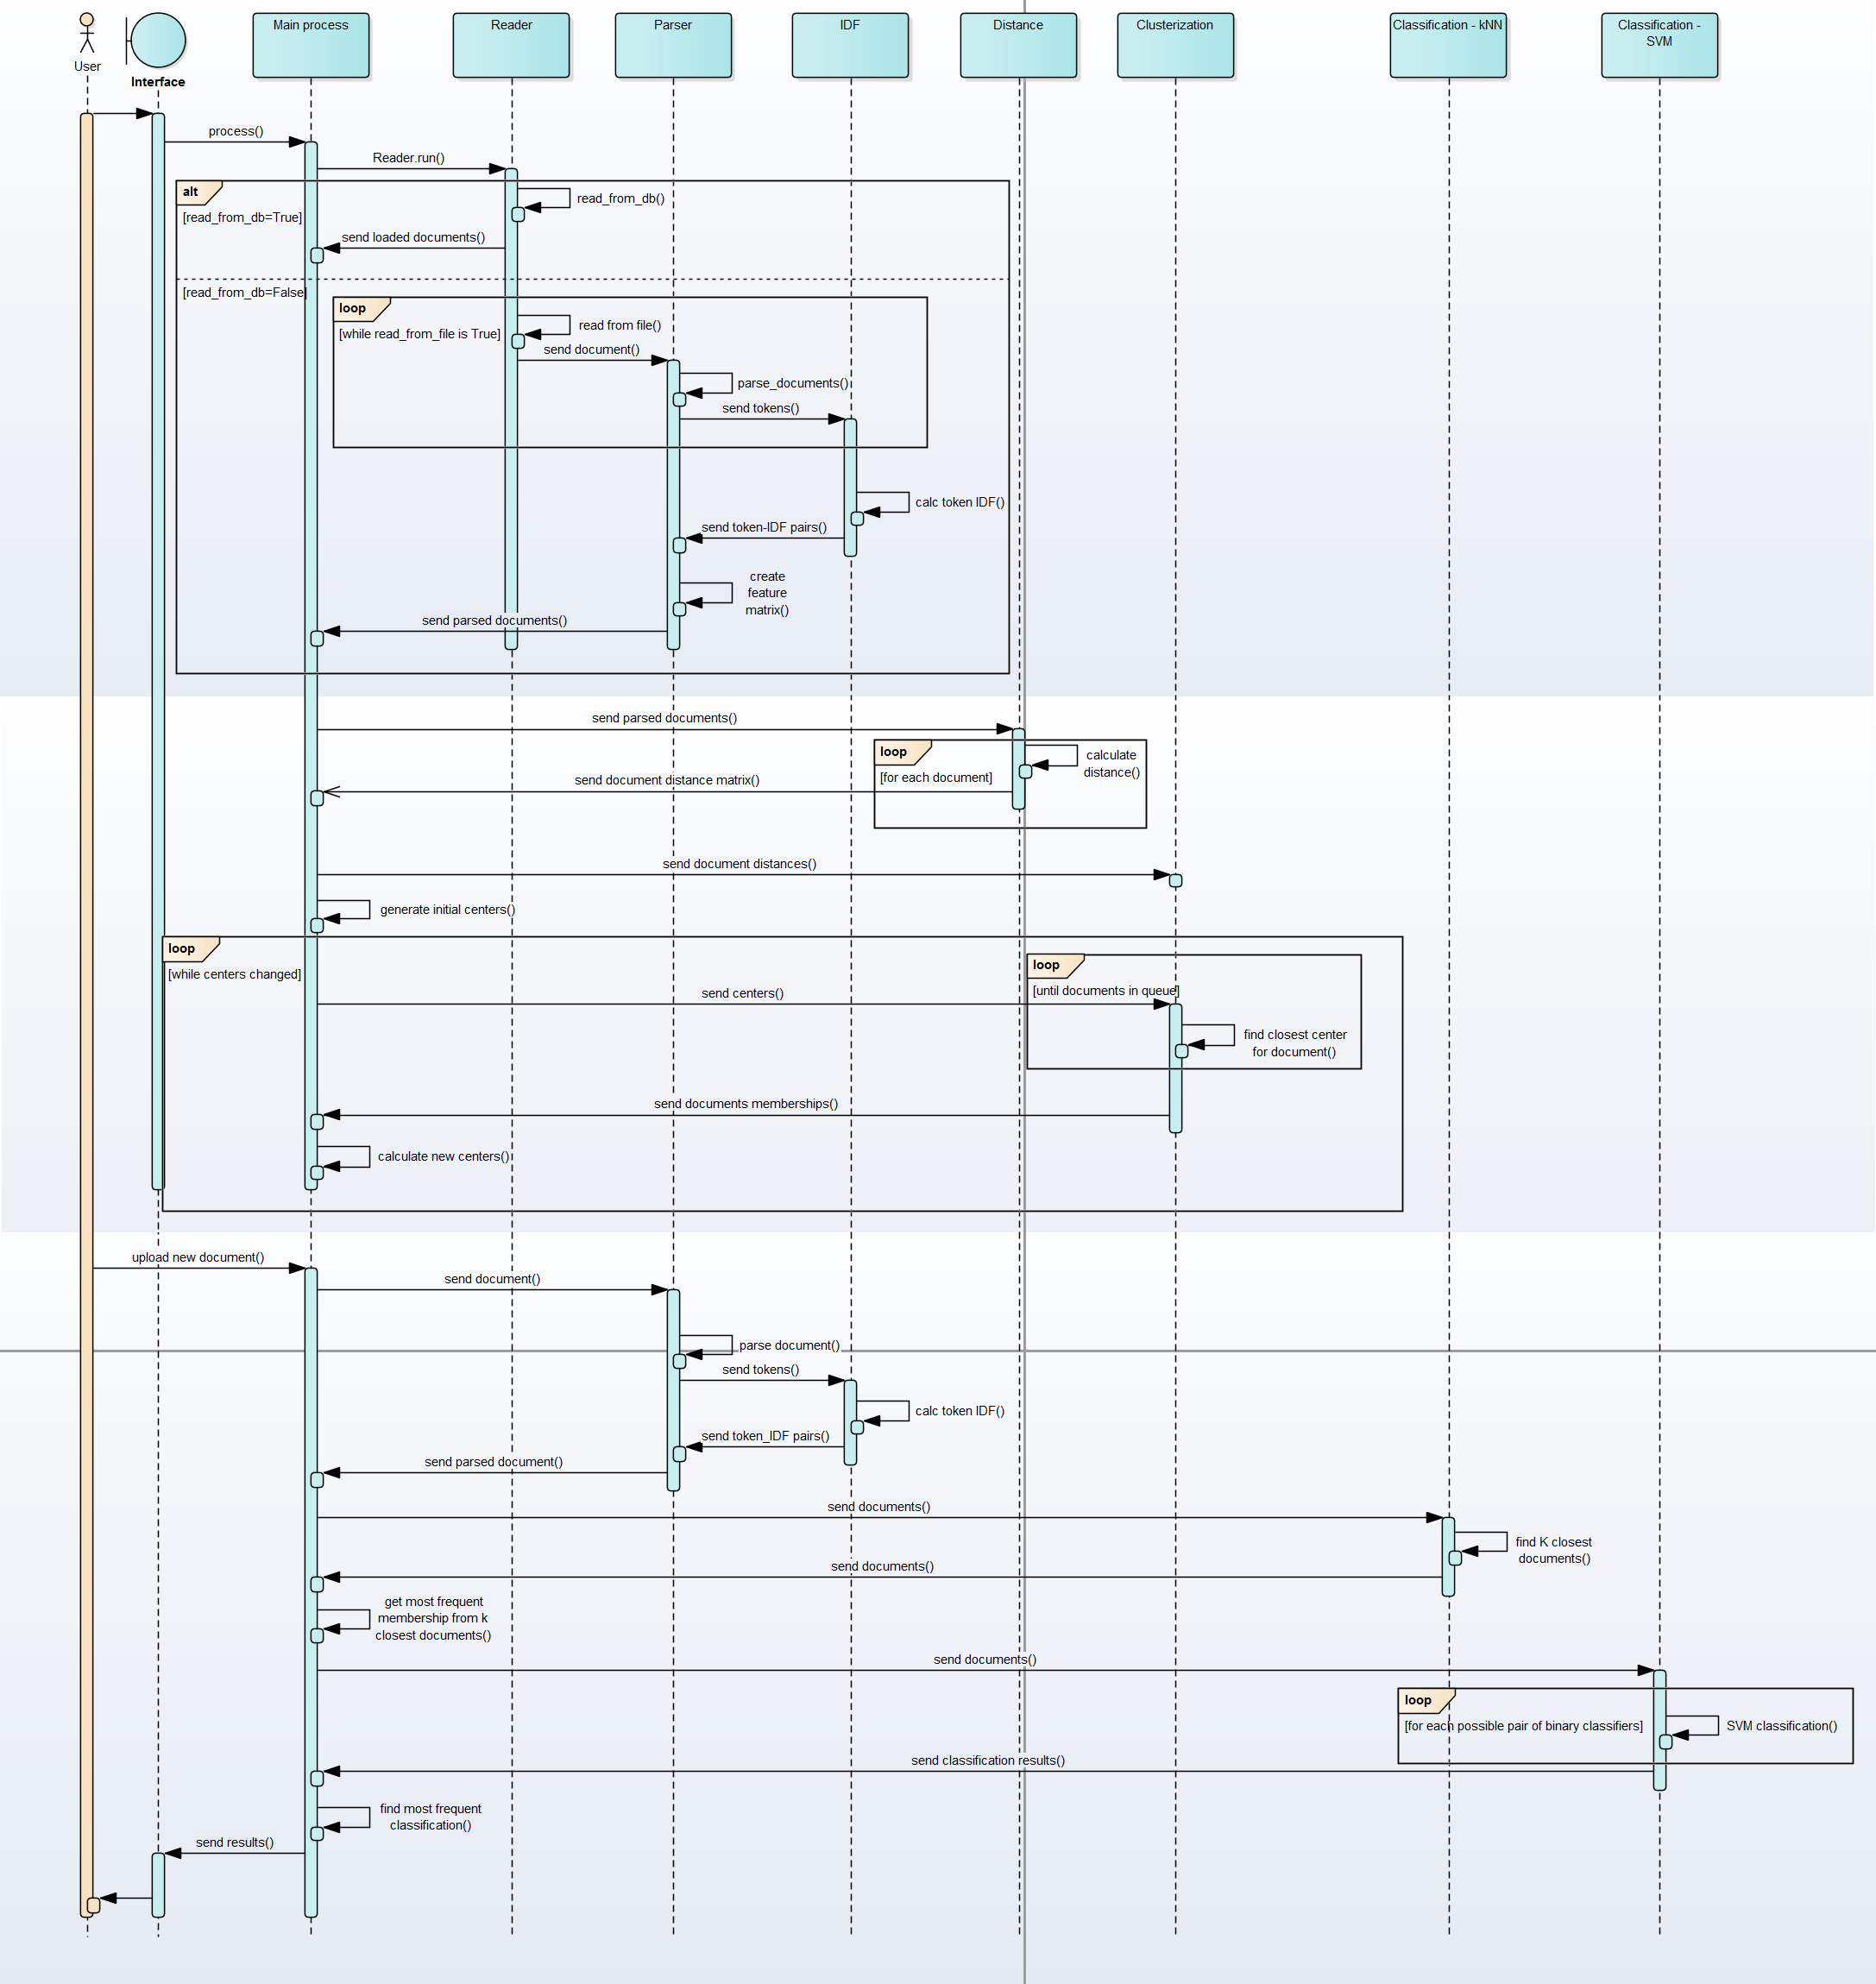
\includegraphics[width=1.2\linewidth]{images/diagrams/seq-full.png}
		\label{appendix-sequence-diagram}
	\end{center}
\end{figure}


\chapter{Instructions}
\section{Installation}
\begin{enumerate}
	\item Install prerequisites: Python 3.5 and git
	\begin{itemize}
		\item https://www.python.org/downloads/release/python-350/
		\item https://git-scm.com/downloads
	\end{itemize}
	\item Clone code repository using command
\begin{lstlisting}[language=Bash, numbers=none]
git clone git@github.com:macsz/parallel-wiki-classifier.git
\end{lstlisting}
	\item To install all required libraries, execute command:
\begin{lstlisting}[language=Bash, numbers=none]
pip install -r source/requirements.txt
\end{lstlisting}
\item Install dictionaries for lemmatization and stop words removal:
\begin{lstlisting}[language=Bash, numbers=none]
python -c "import nltk; nltk.download('stopwords'); nltk.download('wordnet')"
\end{lstlisting}
\end{enumerate}
\section{Usage}

\begin{enumerate}
	\item Download document corpus on which you wish to work on. You can use database dumps of Wikipedia, available at https://dumps.wikimedia.org/enwiki/ . For this purpose you can also use script \textit{./data/download-wiki.sh} included in the repository. It will help you to choose and download proper document corpus.
	
	\item Before running application, please check the content of the configuration file (\textit{wiki\.conf} file in source directory) and change values to your needs. In configuration file you can also point the document you wish to classify.
	
	\item Execute \textit{./run.sh} script to run full flow of application - document parsing, calculating TF-IDF values, calculating distances, clusterization, kNN classification and SVM classification. 
	
	If you wish to run only certain modules of application, you can do this by running:
	\begin{lstlisting}[language=Bash, numbers=none]
	python pwc.py
	\end{lstlisting}
	and appending desired parameters that corresponds to certain modules:
	\begin{itemize}
		\item \textit{--parse} - for document parsing and TF-IDF calculations
		\item \textit{--distance} - for calculating distances
		\item \textit{--cluster} - for clusterizing documents using k-means algorithm
		\item \textit{--classify} - for classification using kNN algorithm
		\item \textit{--svm} - for classification using SVM algorithm
	\end{itemize}
\end{enumerate}